% thesis.tex: Primary TeX control file for thesis.
\documentclass[11pt, oneside]{format/mnthesis}
\usepackage{epsfig}    % Allows the inclusion of eps files
\usepackage{epic}      % Enhanced picture mode
\usepackage{eepic}     % Extensions for epic
\usepackage{units}     % SI unit typesetting
\usepackage{url}       % URL handling
\usepackage{longtable} % Tables that continue onto multiple pages
\usepackage{mathrsfs}  % Support for \mathscr script
\usepackage{multirow}  % Span rows in tables
\usepackage{bigstrut}  % Space struts in tables up and down
\usepackage{amssymb}   % AMS math symbols and helpers
\usepackage{graphicx}  % Enhanced graphics support
\usepackage{setspace}  % Adjust spacing in captions, single by default
\usepackage{xspace}    % Automatically adjusting space after macros
\usepackage{amsmath}   % \text, and other math formatting options
\usepackage{siunitx}   % \num{} formatting and SI unit formatting
\usepackage{booktabs}  % Enhanced tables with \toprule, etc.
\usepackage{hyperref}  % Add clickable links to other parts of the document
\usepackage[noabbrev]{cleveref} % Automatically determine \cref type

% Configure the siunitx package
\sisetup{
    group-separator = {,}, % Use , to separate groups of digits, like 12,345
    list-final-separator = {, and } % Always use the serial comma in \SIlist
}

% Configure the cleveref package
\newcommand{\creflastconjunction}{, and } % Always use the serial comma

% Include the commands from 'definitions.tex'

% Simplifying definitions
\newcommand{\beq}{\begin{equation}}
\newcommand{\eeq}{\end{equation}}

\newcommand{\half}{\tfrac{1}{2}}

\newcommand{\pp}{\phantom{0}}
\newcommand{\PP}{\phantom{00}}


% Add space between rows of tables
\newcommand{\spacerows}[1]{\renewcommand{\arraystretch}{#1}}

\newcolumntype{L}[1]{>{\raggedright\let\newline\\\arraybackslash\hspace{0pt}}m{#1}}
\newcolumntype{C}[1]{>{\centering\let\newline\\\arraybackslash\hspace{0pt}}m{#1}}
\newcolumntype{R}[1]{>{\raggedleft\let\newline\\\arraybackslash\hspace{0pt}}m{#1}}


% Define SI units 
\DeclareSIUnit\fm{fm}
\DeclareSIUnit\lumunits{\per\square\cm\per\second}
\DeclareSIUnit\mAmin{\mA\per\min}
\DeclareSIUnit\torr{Torr}
\DeclareSIUnit\invfb{fb^{-1}}
\DeclareSIUnit\invpb{pb^{-1}}
\DeclareSIUnit\nb{nb}


% Define physics variables
\newcommand{\sC}{\mathrm{C}}
\newcommand{\sP}{\mathrm{P}}
\newcommand{\sT}{\mathrm{T}}
\newcommand{\sCP}{\mathrm{CP}}
\newcommand{\sCPT}{\mathrm{CPT}}

\newcommand{\SUthree}{SU(3)}
\newcommand{\SUtwo}{SU(2)}
\newcommand{\Uone}{U(1)}

\newcommand{\alphaQED}{\alpha}
\newcommand{\alphaQCD}{\alpha_S}

\newcommand{\cRed}{r}
\newcommand{\cGreen}{g}
\newcommand{\cBlue}{b}

\newcommand{\acRed}{\bar{\cRed}}
\newcommand{\acGreen}{\bar{\cGreen}}
\newcommand{\acBlue}{\bar{\cBlue}}


% Define standard model particles
\newcommand{\quark}{q}
\newcommand{\qup}{u}
\newcommand{\qdown}{d}
\newcommand{\qcharm}{c}
\newcommand{\qstrange}{s}
\newcommand{\qbottom}{b}
\newcommand{\qtop}{t}

\newcommand{\aquark}{\bar{\quark}}
\newcommand{\aqup}{\bar{\qup}}
\newcommand{\aqdown}{\bar{\qdown}}
\newcommand{\aqcharm}{\bar{\qcharm}}
\newcommand{\aqstrange}{\bar{\qstrange}}
\newcommand{\aqbottom}{\bar{\qbottom}}
\newcommand{\aqtop}{\bar{\qtop}}

\newcommand{\lepton}{l}
\newcommand{\lel}{e^-}
\newcommand{\lmu}{\mu^-}
\newcommand{\ltau}{\tau^-}
\newcommand{\neutrino}{\nu}
\newcommand{\vel}{\nu_{e}}
\newcommand{\vmu}{\nu_{\mu}}
\newcommand{\vtau}{\nu_{\tau}}

\newcommand{\alepton}{\bar{\lepton}}
\newcommand{\alel}{e^+}
\newcommand{\almu}{\mu^+}
\newcommand{\altau}{\tau^+}
\newcommand{\aneutrino}{\bar{\neutrino}}
\newcommand{\avel}{\bar{\ve}}
\newcommand{\avmu}{\bar{\vmu}}
\newcommand{\avtau}{\bar{\vtau}}

\newcommand{\fermion}{f}
\newcommand{\afermion}{\bar{\fermion}}

\newcommand{\W}{W}
\newcommand{\Z}{Z}
\newcommand{\photon}{\gamma}
\newcommand{\gluon}{g}
\newcommand{\Higgs}{H}


% Define hadrons 
\newcommand{\jpsi}{J/\psi}
\newcommand{\psip}{\psi(2S)}
\newcommand{\apsip}{\psi(3686)}
\newcommand{\psipp}{\psi(3770)}

\newcommand{\D}{D}
\newcommand{\aD}{\overline{D}}
\newcommand{\Dp}{D^+}
\newcommand{\Dm}{D^-}
\newcommand{\DO}{D^0}
\newcommand{\aDO}{\overline{\DO}}


\newcommand{\pip}{\pi^+}
\newcommand{\pim}{\pi^-}
\newcommand{\pipm}{\pi^\pm}
\newcommand{\piO}{\pi^0}
\newcommand{\Kp}{K^+}
\newcommand{\Km}{K^-}
\newcommand{\Kpm}{K^\pm}
\newcommand{\Ks}{K^0_S}

% Define particle pairs
\newcommand{\ee}{\alel\lel}
\newcommand{\mumu}{\almu\lmu}
\newcommand{\tautau}{\ltau\altau}
\newcommand{\qqbar}{\quark\aquark}
\newcommand{\ffbar}{\fermion\afermion}
\newcommand{\DDbar}{\D\aD}
\newcommand{\twophoton}{\photon\photon}


% Define particle variables
\newcommand{\xsecDDbar}{\sigma_{\DDbar}}

\newcommand{\Mpsipp}{M^{\psipp}}
\newcommand{\Gpsipp}{\Gamma^{\psipp}}
\newcommand{\Geepsipp}{\Gamma_{ee}^{\psipp}}
\newcommand{\Ppsipp}{\phi^{\psipp}}
\newcommand{\Gpsip}{\Gamma^{\psip}}
\newcommand{\Geepsip}{\Gamma_{ee}^{\psip}}
\newcommand{\GeepsipptoDD}{\Gamma_{ee}^{\psipptoDD}}


% Define detector / collider variables
\newcommand{\DeltaE}{\Delta E}
\newcommand{\mbc}{m_{\text{BC}}}
\newcommand{\Ecm}{E_{\text{cm}}}
\newcommand{\Ebeam}{E_{\text{beam}}}
\newcommand{\Etag}{E_{\text{tag}}}
\newcommand{\ptag}{\vec{p_{\text{tag}}}}
\newcommand{\minv}{m_{\text{inv}}}
\newcommand{\dEdx}{\frac{dE}{dx}}
\newcommand{\tdEdx}{dE/dx}
\newcommand{\lum}{\mathcal{L}}
\newcommand{\Dtag}{D\text{-tag}}
\newcommand{\DTagAlg}{\texttt{DTagAlg}}


% Define derivation variables
\newcommand{\BDD}{\mathcal{B}_{\DDbar}}
\newcommand{\BnDD}{\mathcal{B}_{n\DDbar}}
\newcommand{\zDD}{z_{\Dp\Dm}}
\newcommand{\Nprop}{N_{\text{prop}}}
\newcommand{\Ngen}{N_{\text{gen}}}


% Define decay modes
\newcommand{\psipptoDD}{\psipp \rightarrow \DDbar}
\newcommand{\bhabha}{\ee \rightarrow \ee}

\newcommand{\DOmodeA}{\DO \rightarrow \Km \, \pip}
\newcommand{\DOmodeB}{\DO \rightarrow \Km \, \pip \, \piO}
\newcommand{\DOmodeC}{\DO \rightarrow \Km \, \pip \, \pip \, \pim}

\newcommand{\DpmodeA}{\Dp \rightarrow \Km \, \pip \, \pip}
\newcommand{\DpmodeB}{\Dp \rightarrow \Km \, \pip \, \pip \, \piO}
\newcommand{\DpmodeC}{\Dp \rightarrow \Ks \, \pip}
\newcommand{\DpmodeD}{\Dp \rightarrow \Ks \, \pip \, \piO}
\newcommand{\DpmodeE}{\Dp \rightarrow \Ks \, \pip \, \pip \, \pim}
\newcommand{\DpmodeF}{\Dp \rightarrow \Kp \, \Km  \, \pip}




\linespread{1.3}

% Compile only the chapters listed here
\includeonly{
    sections/default/title,
    sections/default/conclusion,
    sections/main/01_intro,
    sections/main/02_theory,
    sections/main/03_detector,
    sections/main/04_software,
    sections/appendix/A1_glossary,
}

\begin{document}

% Set the bibliography style
\bibliographystyle{format/hunsrt}

% Title and other sections that come before the body of the document
%%%%%%%%%%%%%%%%%%%%%%%%%%%%%%%%%%%%%%%%%%%%%%%%%%%%%%%%%%%%%%%%%%%%%%%%%%%%%%%%
% title.tex - Set up the beginning of thesis.
%%%%%%%%%%%%%%%%%%%%%%%%%%%%%%%%%%%%%%%%%%%%%%%%%%%%%%%%%%%%%%%%%%%%%%%%%%%%%%%%

% Uncomment to turn on draft mode, which changes the title page to have a draft
% label and date of compilation
%\draft

% Set the type of thesis
\phd % use if for a Ph.D. dissertation
%\ms % use if for a Master of Science thesis

% Set the title and your name. Remember that the guidelines state:
%
% "The title of the thesis must not contain chemical or mathematical formulas,
% symbols, superscripts, subscripts, Greek letters, or other non-standard
% characters; words must be substituted."
\title{\bf Thesis Title}
\author{Full Author Name}
% Advisor name, put co-advisors here as well separated by commas
\director{Name of the Advisor}

% Specify the month and year; if commented out then these default to the
% current month and year
\submissionmonth{May}
\submissionyear{2015}

% Pages after the title page
\abstract{%%%%%%%%%%%%%%%%%%%%%%%%%%%%%%%%%%%%%%%%%%%%%%%%%%%%%%%%%%%%%%%%%%%%%%%%%%%%%%%%
% abstract.tex: Abstract
%%%%%%%%%%%%%%%%%%%%%%%%%%%%%%%%%%%%%%%%%%%%%%%%%%%%%%%%%%%%%%%%%%%%%%%%%%%%%%%%

%%%%%%%%%%%%%%%%%%%%%%%%%%%%%%%%%%%%%%%%%%%%%%%%%%%%%%%%%%%%%%%%%%%%%%%%%%%%%%%%
}

% Copyright: Uncomment one of the following:
\copyrightpage       % Full copyright
%\copyrightpageccby   % Full copyright with Creative Commons CC-BY 4.0 license
%\copyrightpageccbysa % Full copyright with Creative Commons CC-BY-SA 4.0 license

% Acknowledgments and dedication
\acknowledgements{%%%%%%%%%%%%%%%%%%%%%%%%%%%%%%%%%%%%%%%%%%%%%%%%%%%%%%%%%%%%%%%%%%%%%%%%%%%%%%%%
% acknowledge.tex: Acknowledgements
%%%%%%%%%%%%%%%%%%%%%%%%%%%%%%%%%%%%%%%%%%%%%%%%%%%%%%%%%%%%%%%%%%%%%%%%%%%%%%%%

There are many people that have earned my gratitude for their contribution to my
time in graduate school.

%%%%%%%%%%%%%%%%%%%%%%%%%%%%%%%%%%%%%%%%%%%%%%%%%%%%%%%%%%%%%%%%%%%%%%%%%%%%%%%%
}
\dedication{This is where the Dedications go!}

% Use a special preface
%\extra{\input{preface}}

% The \beforepreface command actually causes insertion of the title,
% abstract, signature, and copyright pages into the new document.
\beforepreface

% Define the text to go before the table of contents
\figurespage
\tablespage

% The \afterpreface command actually causes insertion of the
% contents, list of figures, etc. into the new document.
\afterpreface
%%%%%%%%%%%%%%%%%%%%%%%%%%%%%%%%%%%%%%%%%%%%%%%%%%%%%%%%%%%%%%%%%%%%%%%%%%%%%%%%


% Now lets include the body of the document...
\chapter{Introduction}
\label{ch_intro}


Since the discovery of the $\jpsi$ particle in 1974, the charm energy range (\SIrange{3.0}{4.5}{\GeV}) has been one of the most precisely studied regions in particle physics.
This has led to the further discovery of many more resonances, as shown in \Cref{fig:R_scan}.

\begin{figure}[H]
\centering
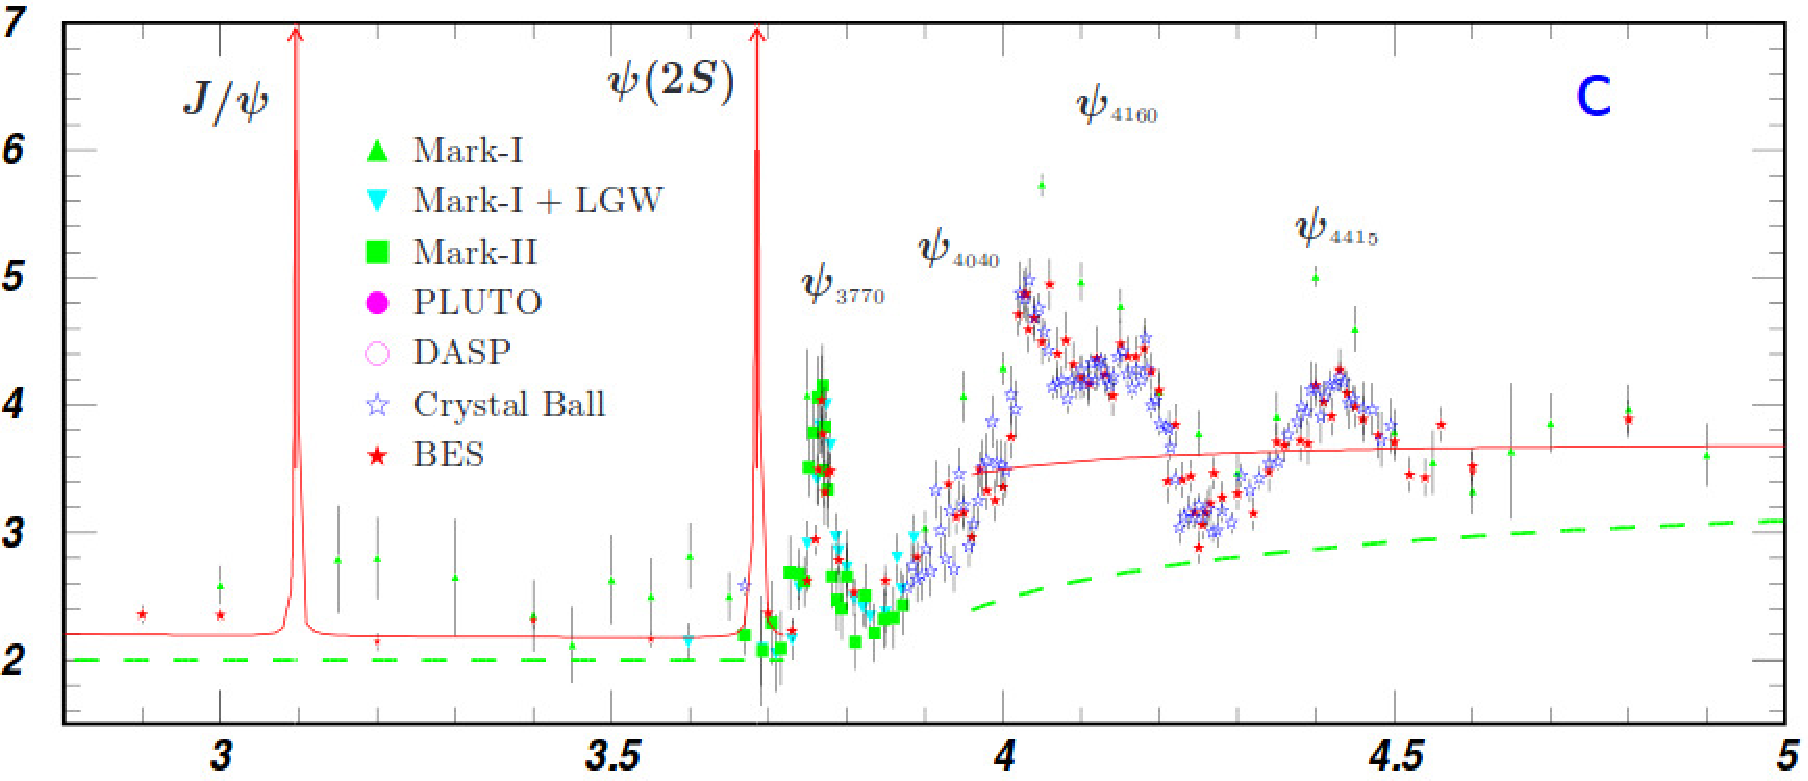
\includegraphics[scale=0.50]{figures/images/R_scan.pdf}
\caption{Measurements of $R = \sigma(\ee \rightarrow \text{hadrons}) / \sigma(\ee \rightarrow \mumu)$.}
\label{fig:R_scan}
\end{figure}

Many of the lower mass resonances are predictable within the context of the quark model.
However, there are a number of states which have been predicted, but not yet discovered.
There are also states which were discovered experimentally without any corresponding predictions.
A variety of these particles are shown in \Cref{fig:charmonia}.

\begin{figure}[H]
\centering
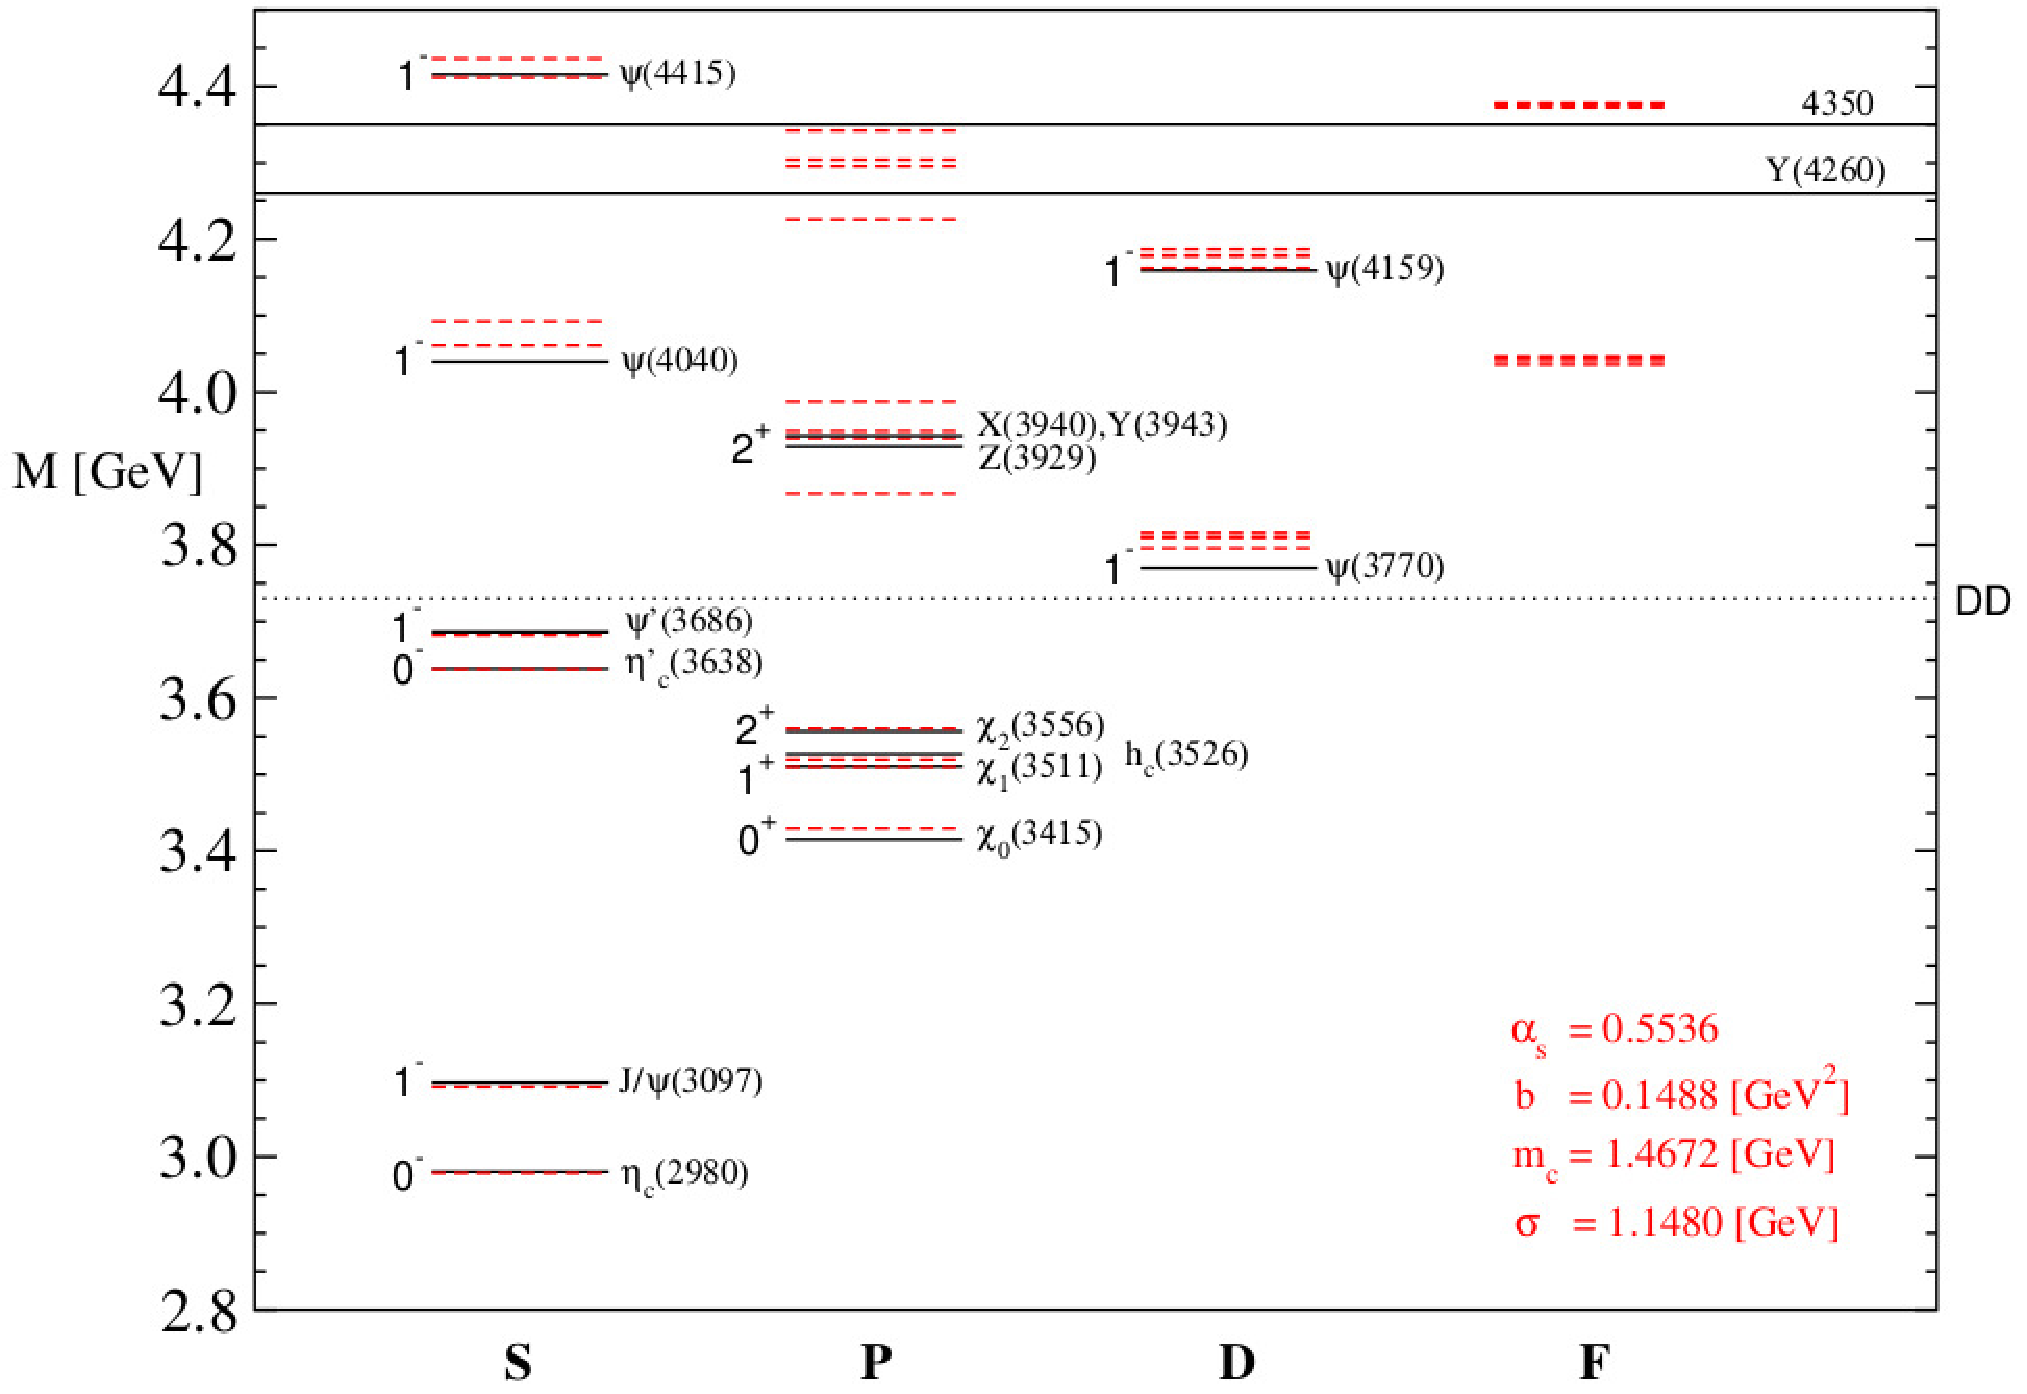
\includegraphics[scale=0.40]{figures/images/charmonia.pdf}
\caption{Measured and predicted charmonium resonances.}
{Solid black lines represent measurements while the dashed red lines are predictions.}
\label{fig:charmonia}
\end{figure}

The resonances below the $\DDbar$ threshold, like the $\jpsi$ and the $\psip$, show solid agreement with their theoretical predictions.
However, many of the ones above, such as the $\psipp$, still show some disagreement.
This is likely due to the more complicated interactions introduced from $\DDbar$ decays.
Several experiments have attempted to measure the shape of the $\psipp$ based on different assumptions.
The most prominent of these is the assumption of interference.
This can have notable effects on the resultant parameters of the $\psipp$, such as the mass, shown in \Cref{tab:previous_results}.

\begin{table}[H]
\centering
\begin{tabular}{c l|c l}
\hline
\multicolumn{2}{c|}{$\Mpsipp$ [\si{\MeV}] (No Interference)} & \multicolumn{2}{c}{$\Mpsipp$ [\si{\MeV}] (With Interference)} \\ [1pt] 
\hline
BES-II \cite{ref:Ablikim:2007}   & 3772.0 $\pm$ 1.9           & BaBar \cite{ref:Aubert:2008b} & 3778.8 $\pm$ 1.9 $\pm$ 0.9 \\
Belle  \cite{ref:Brodzicka:2008} & 3776.0 $\pm$ 5.0 $\pm$ 4.0 & KEDR  \cite{ref:Anashin:2012} & $3779.2^{+1.8 \, +0.5 \, +0.3}_{-1.7 \, -0.7 \, -0.3}$ \\ 
BaBar  \cite{ref:Aubert:2008a}   & 3775.5 $\pm$ 2.4 $\pm$ 0.5 & & \\
\hline
\end{tabular}
\caption{Previous experimental results for the mass of the $\psipp$.}
{Where applicable, the first errors are statistical, the second are systematic, and the third are model-dependent.}
\label{tab:previous_results}
\end{table}

Both BaBar \cite{ref:Aubert:2008b} and KEDR \cite{ref:Anashin:2012} found it necessary to include interference effects for fitting the $\DDbar$ spectrum.
However, the statistics of the KEDR sample were insufficient to fully resolve the discrepancies seen with other experiments that ignored interference.
{\bf Using the larger data sample available at BESIII, we have precisely measured and analyzed the shape of the $\DDbar$ spectrum around the $\psipp$ resonance.}
We have also used this measurement to probe the branching fraction of $\nonDDbar$ decays in this region.


\section{Procedure}
\label{sec:procedure}

The basis of this measurement involves identifying $\DDbar$ pairs which have decayed from $\psipp$.
All data used in this analysis was collected from $\ee$ collisions analyzed by the BESIII detector.
As $\lel$ and $\alel$ are fundamental particles, the total energy of each is transferred in the collision.
Additionally, the ability to precisely tune these two beam energies allows for the targeted production of specific particles, such as the $\psipp$.
However, resonances like this will decay almost instantaneously.
For example, the $\psipp$ has an average lifetime of ${\sim}\SI{e-23}{\s}$.
Even if it were traveling at $c$, the farthest distance this could travel would be $(\SI{3e8}{m/s}) \times ({\sim}\SI{e-23}{\s}) \approx \SI{1}{\fm}$.
This distance, approximately the radius of a proton, is far too small to be resolved by our detectors.
Even the initial decay into $\DDbar$ pairs is too small to precisely measure, as their lifetime of \SI{~4e-13}{\s} corresponds to a maximum distance of ${\sim}\SI{1}{\mm}$ if it were traveling at $c$.
However, the limited available energy in these decays ($m_{\psipp} - 2 \times m_{D} \approx \SI{40}{\MeV})$ means the velocity is much, much slower.

% \tau = 1 / 25 [1/MeV] * (200 MeV / 1e-15 m) / (3e8 m / s) = 200 / (3 * 25) e-23 s ~ 10^-13 s

Instead, the reconstruction of candidate $D$ particles relies on measuring their decays into other known modes.
While there are dozens of possible decays modes, we focus on those which have high branching fractions, and are comprised of particles identifiable by the BESIII detector.
For our purposes, these are $\pipm, \Kpm, \piO,$ and $\Ks$.
Each of these particles leave `tracks' within the detector; charged particles travel along curved paths and interact electromagnetically with charged wires along their trajectory, while neutral particles travel along straight paths and deposit bursts of energy after contacting crystals located along the inner walls of the detector.
The various components of the BESIII detector analyze these tracks to determine the type of particle, as well as its momentum and energy.
By analyzing sets of particles corresponding to the chosen decay modes, we can reconstruct the combination most likely to have originated from a $D$ based on their total energy.


To determine the $\psipptoDD$ cross section, we need to count the number of $\DDbar$ pairs produced, as well as measure the integrated luminosity, at each energy point in our data sample.
This counting is done not only for the actual collision data collected, but also for computed generated Monte Carlo (MC) background samples.
Each of these backgrounds corresponds to a particular event type which may be mistaken as signal, such as $\ee \rightarrow \tautau$.
We subtract these misidentified contributions from the total amount found in data to determine the actual number of reconstructed $\DDbar$ events.
Also from MC, we calculate the efficiency of reconstructing $\DDbar$ decays based on our selection criteria.
By dividing the actual reconstructed events by this efficiency, we identify the true number of $\DDbar$ events produced.
Then, using the measured luminosity for each energy point, we determine the cross section as a function of center-of-mass energy.

% 
% While energy and momentum conservation remain fundamental laws of physics, accounting for the 
% 
% Also must correct for initial state radiation
% Accelerated particles (such as those traveling around a circular collider) radiate energy
% This energy reduces the total amount available in a collision
% Can lead to producing lower resonances (jpsi, psip) instead of targeted psipp
% Also decreases total energy available at each point, and must be accounted for
% Effect is very calculable, and included in cross section derivation


The specific details of this analysis start with background on relevant theoretical concepts.
Next, we list the specifications for the collider and detector which collected the data used for these measurements along with their related analysis software and reconstruction methods. 
From here, we further describe the procedure for determining the $\psipptoDD$ cross section and show the results with systematic uncertainties.
Finally, we examine the current progress of measuring the $\nonDDbar$ branching fraction.



%% Base Chapters
\chapter{Theoretical Background}
\label{ch:theory}

\section{Standard Model}
\label{sec:standard_model}

Developed throughout the 1960s and 1970s, the Standard Model provides the most complete description of observable matter in the universe to date.
It is a classification of all confirmed subatomic particles currently known, and predicts the most accurate results of any scientific theory ever measured.
Each of the electromagnetic, weak, and strong fundamental forces are well described by this formulation.
These three are described by an $\SUthree \times \SUtwo \times \Uone$ group, where the $\SUthree$ corresponds to the strong force, the $\SUtwo$ corresponds to the weak force, and the $\Uone$ corresponds to the electromagnetic force.
The remaining fundamental force, gravity, is not included in the Standard Model.
It is negligible on the scale of the masses of fundamental particles, and will be ignored in the discussions that follow.


\subsection{Electromagnetic Force}
\label{ssec:electromagnetic}

The electromagnetic force is responsible for the forces between objects with electric charge, most notably binding together electrons and protons to form atoms and the structures they comprise.
The theory of electromagnetic interactions is known as Quantum Electrodynamics (QED).
Within this theory, the mediator of this force is the photon, a massless vector boson.
As there is only a single mediator, and a single conserved quantity (electric charge), the formulation of QED is relatively simple compared to the other forces.
Still, the predictions it makes show astounding consistency with experiment, such as correctly calculating the anomalous magnetic dipole moment of the electron to more than 10 significant figures.
Much of this success is due to QED being calculable through perturbation theory, where corrections are applied in terms of higher order factors of the coupling constant, $\alphaQED$.
This is possible due to its relatively small value ($\alphaQED \approx 1/137$), as the terms are convergent below very high orders of $\alphaQED$. 

\subsection{Weak Force}
\label{ssec:weak}

The weak force is responsible for radioactive decay and other subatomic phenomena.
This is distinct from the electromagnetic and strong interactions, where the constituent particles cannot change their types (or flavors).
The mediators of this force are the $\W$ and $\Z$, which are massive vector bosons.
Not only are each of their masses non-zero, they are extremely heavy particles at \SIlist{80.4;90.2}{\GeV}, respectively \cite{ref:Olive:2014}.
These large masses not only limit the interaction distance of the weak force, but also minimize the interaction strength (which is inversely proportion to mass).
Furthermore, the large $\W$ and $\Z$ masses also lead to much slower interaction times, further reducing the effects of the weak force in comparison to the strong and electromagnetic forces.


In addition to transforming particle flavor, the weak force is also unique in its violation of various symmetries.
The first discovery of symmetry violation came in 1957, when Wu and others \cite{ref:Wu:1957} discovered the weak force did not behave identically under parity ($\sP$) transformations (i.e., mirror reflection).
To account for this, a new theory conserving a compound symmetry was proposed.
This combined charge conjugation ($\sC$), the swapping of particles with their antiparticles, with parity to form $\sCP$ parity.
However, in 1964, evidence of $\sCP$ violation was also discovered by Cronin and Fitch \cite{ref:Christenson:1964}.
The resolution to this symmetry conservation involves yet a third symmetry, time reversal ($\sT$), in which time is replaced with its negative ($t \rightarrow -t$).
While the weak force violates these symmetries individually, the application of all three ($\sCPT$) is conserved across all known processes, and is known as the $\sCPT$ Theorem.


At higher energy scales, the electromagnetic and weak forces unify into the electroweak force.
In this theory, there are initially four massless gauge bosons mediating the interactions.
As a result of the Higgs mechanism, the initial gauge symmetry is broken at lower energies, and three of these bosons acquire a mass.
These three bosons are the $\W^\pm$ and $\Z$, while the remaining massless boson is the $\photon$.
The energies scales required for this unification were only present in the early universe.
Before this, it is also believed there was an epoch of even higher energy, in which the electroweak force merged with the strong force.


\subsection{Strong Force}
\label{ssec:strong}

The strong force is responsible for binding together particles known as hadrons.
The theory of strong interactions is known as Quantum Chromodynamics (QCD).
Like the electromagnetic force, the mediator of the strong force is also a massless vector boson, the gluon.
However, while massless particles typically correspond to an infinite interaction range, the strong potential becomes very large at higher separations.
This prevents particles which interact through the strong force, known as quarks (see \Cref{sssec:fermions}), from existing as isolated entities in a process known as confinement.
The typical interaction range is on the order of the proton radius, around \SI{e-15}{\m}.
QCD calculations face serious challenges, however, as the coupling constant is not small ($\alphaQCD \gtrsim 1$).
This excludes the use of perturbation theory for most cases, as the higher order terms do not converge.


Strong interactions are associated with a corresponding conserved quantity known as the color charge. 
Despite its name, however, the term 'color' has no association with light, which is a purely electromagnetic phenomena.
There are three colors associated with this charge, red ($\cRed$), green ($\cGreen$), and blue ($\cBlue$).
For anti-particles, there are oppositely charged values ($\acRed, \acGreen,$ and $\acBlue$).
In order for hadrons to be formed, the total color values of the constituents must be colorless.
This means the total sum must involve all three colors ($\cRed \cGreen \cBlue$ or $\acRed \acGreen \acBlue$) or pairs of opposite colors ($\cRed \acRed, \cGreen \acGreen, $ or $\cBlue \acBlue$).
However, these individual colors are not observable in nature.
Because particles with different color values are distinct, this effectively triples the number of possible particle combinations, due to combinatorics.


Unlike the photon, which does not carry an electric charge, gluons do possess a color charge.
There are eight possible color combinations which a gluon may possess, which are typically expressed using the Gell-Mann representation of $\SUthree$.
With this basis, each gluon is linearly independent, and no combination of gluons can be used to form a color singlet state.
This non-zero charge of the force carrier makes QCD significantly more complex than QED.
In fact, carrying color charge means gluons can also interact with each other directly, leading to certain theoretical states such as glueballs. 


\subsection{Elementary Particles}
\label{ssec:elementary_particles}

There are two primary groups contained in the Standard Model, fermions and bosons. 
This division is based on the Spin Statistics theorem, where fermions (bosons) have half-integer (integer) spins.
As described by the Pauli Exclusion principle, nature restricts fermions from occupying the same quantum state.
Bosons, however, do not have this restriction, and can have any number occupying the same state.

\begin{figure}[H]
\centering
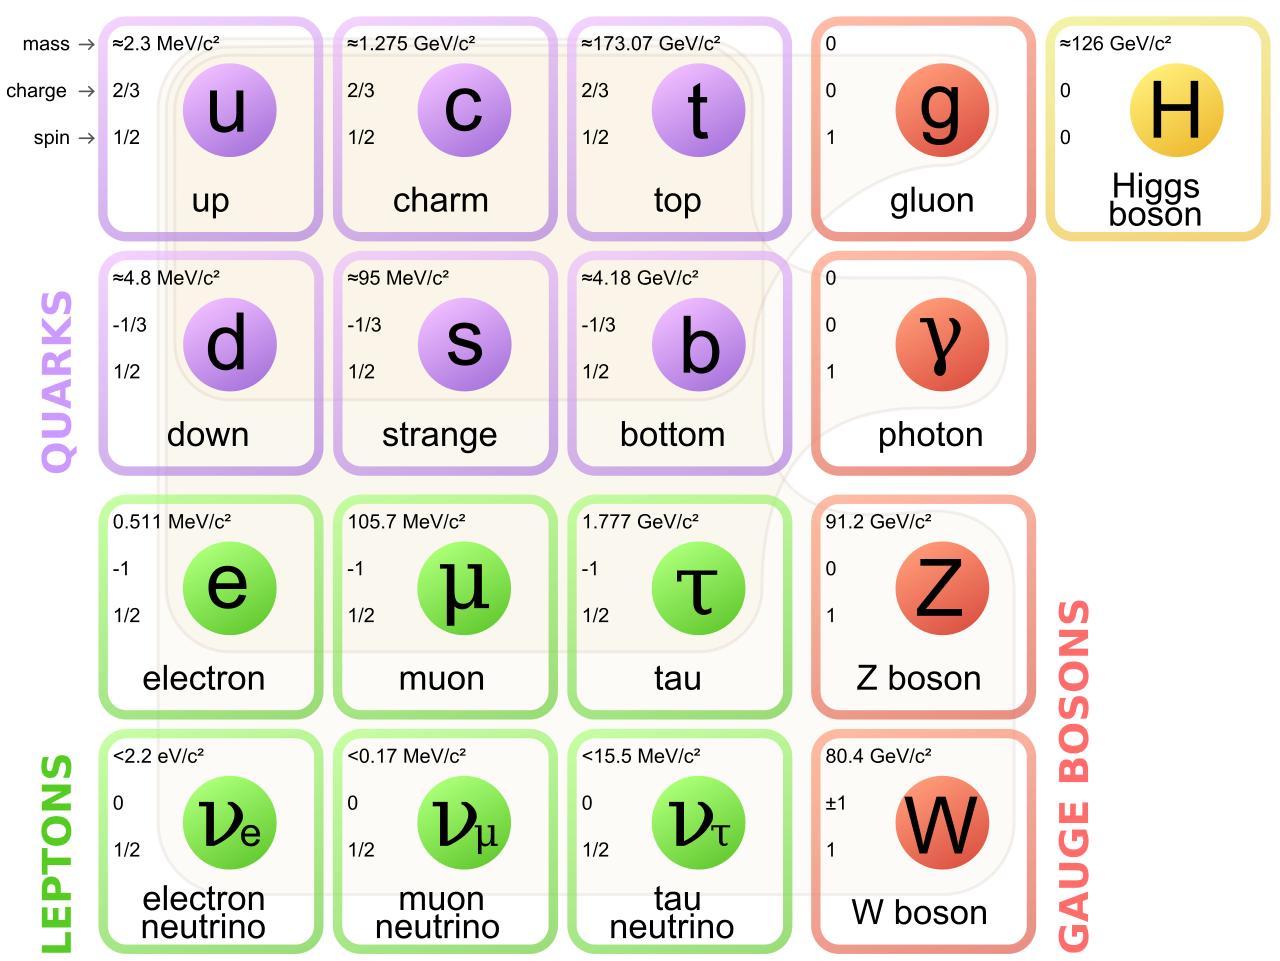
\includegraphics[scale=0.30]{figures/images/standard_model.png}
\caption{The standard model of particle physics.}
{It is comprised of two main groups: fermions, which includes the quarks and leptons, and bosons, which includes the gauge bosons and the Higgs boson. Image reproduced courtesy of \cite{ref:Wikimedia:2006}. }
\label{fig:standard_model}
\end{figure}


\subsubsection{Fermions}
\label{sssec:fermions}

The fermions are divided by their interaction types into two major groups, quarks ($\quark$) and leptons ($\lepton$).
Each of these groups contains six particles with their corresponding antiparticles.
These can be grouped into three generations, which aligns particles with the same electric charges, but greatly differing masses.  
As an example, the up ($\qup$), charm ($\qcharm$), and top ($\qtop$) quarks all have an electric charge of +2/3 (in terms of the electron charge, $e$), but $\qtop$ is approximately five orders of magnitude more massive than $\qup$.
For the quarks and fermions in \Cref{fig:standard_model}, rows indicate particles with the same electric charge, while columns represent each generation of particles.


Although all fermions interact both electromagnetically and weakly, only the quarks interact strongly.
Because of confinement, quarks cannot exist as isolated particles, and are only found in nature as groups of particles called hadrons.
The most common types of hadrons exist as quark-antiquark pairs, known as mesons, or as groups of three quarks (or antiquarks), known as baryons.
There are, however, indications of more exotic combinations of quarks, such as tetra- ($\quark\quark\aquark\aquark$) or penta-quark ($\quark\quark\quark\quark\aquark$) states seen by recent experiments \cite{ref:Ablikim:2013,ref:Liu:2013,ref:Aaij:2015}.


While the negatively charged quarks ($\qdown, \qstrange$, and $\qbottom$) are labeled as definite states, the quarks are actually mixed states.
Through weak interactions, each of these quarks can transform into other quarks.
The probabilities for these transformations are expressed by the Cabibbo-Kobayashi-Maskawa (CKM) Matrix \cite{ref:Kobayashi:1973}, shown in \Cref{fig:ckm_matrix}.
From the experimentally measured values \cite{ref:Olive:2014}, is it evident the matrix is nearly diagonal.
It is also clear that correlations are strongest within each generation, as the off-diagonal terms are generally smaller than the diagonal ones.
Additionally, though the convention splits the negatively charged quarks into mixed states (leaving the positively charged quarks fixed), this choice has no physical basis.
The reverse choice of having mixed positively charged quarks is equivalent.

\begin{figure}[H]
\centering
$
\begin{bmatrix}
   |V_{ud}| & |V_{us}| & |V_{ub}| \\
   |V_{cd}| & |V_{cs}| & |V_{cb}| \\
   |V_{td}| & |V_{ts}| & |V_{tb}| \\
\end{bmatrix}
=
\begin{bmatrix}
    0.97427 \pm 0.00014 & 0.22536 \pm 0.00061 & 0.00355 \pm 0.00015 \\
    0.22522 \pm 0.00061 & 0.97343 \pm 0.00015 & 0.0414  \pm 0.0012  \\
    0.00886^{+0.00033}_{-0.00032} & 0.0405^{+0.0011}_{-0.0012} & 0.99914 \pm 0.00005 \\
\end{bmatrix}
$
\caption{The Cabibbo-Kobayashi-Maskawa (CKM) Matrix.}
\label{fig:ckm_matrix}
\end{figure}

The values of the CKM matrix are typically parameterized using three Euler angles ($\theta_{12}, \theta_{23}, \theta_{13}$) and a $\sCP$-violating phase parameter ($\delta_{13}$), where the indices represent the three generations of quarks.
This formulation allows the matrix to be cast in the ``standard'' parametrization, shown in \Cref{fig:ckm_standard}.
The form with three separated matrices clearly shows the connections between each generation of quarks.
Namely, the third shows the original formulation in terms of a single rotation, the Cabbibo angle ($\theta_{12}$).
This theory is known as the Glashow-Iliopoulos-Maiani (GIM) mechanism [\cite{ref:Glashow:1970} and was used to explain the suppression of flavor-changing neutral currents (FCNC) before the discovery of the charm quark.
% Current measurements for the standard parameters are $\theta_{12} = \ang{13.04 \pm 0.05}, \; \theta_{13} = \ang{0.201 \pm 0.011}, \; \theta_{23} = \ang{2.38 \pm 0.06}$ and $\delta_{13} = \SI{1.20 \pm 0.08}{\rad}$.

\begin{figure}[H]
\centering
$
    \begin{bmatrix}
        1 &  0      & 0      \\
        0 &  c_{23} & s_{23} \\
        0 & -s_{23} & c_{23} \\
    \end{bmatrix}
    \begin{bmatrix}
         c_{13}                  & 0 & s_{13} e^{-i\delta_{13}}  \\
         0                       & 1 & 0                         \\
        -s_{13} e^{i\delta_{13}} & 0 & c_{13}                    \\
    \end{bmatrix}
    \begin{bmatrix}
         c_{12} & s_{12} & 0 \\
        -s_{12} & c_{12} & 0 \\
         0      & 0      & 1 \\
    \end{bmatrix}
\linebreak
=
    \begin{bmatrix}
          c_{12} c_{13} 
       &  s_{12} c_{13}
       &  s_{13} e^{-i\delta_{13}} \\
         -s_{12} c_{23} - c_{12} s_{23} s_{13} e^{i\delta_{13}}
       &  c_{12} c_{23} - s_{12} s_{23} s_{13} e^{i\delta_{13}}
       &  s_{23} c_{13} \\
          s_{12} s_{23} - c_{12} c_{23} s_{13} e^{i\delta_{13}}
       & -c_{12} s_{23} - s_{12} c_{23} s_{13} e^{i\delta_{13}}
       &  c_{23} c_{13} \\
    \end{bmatrix}
$
\caption{The standard form of the Cabibbo-Kobayashi-Maskawa (CKM) Matrix.}
    {The parameterization is in terms of three angles ($\theta_{12}, \theta_{23}, \theta_{13}$) and a phase angle ($\delta_{13}$). Here, $c_{ij} = \cos\theta_{ij}$ and $s_{ij} = \sin\theta_{ij}$.} 
\label{fig:ckm_standard}
\end{figure}

The leptons are also organized into generations consisting of particles with two distinct charges.
The electron ($\lel$), muon ($\lmu$), and tau ($\ltau$) are all negatively charged particles.
There is also a neutral particle, a neutrino ($\neutrino$), corresponding to each of the charged leptons ($\vel, \vmu, \vtau$).
These are very small mass ($< \SI{1}{\eV}$) particles with extremely low interactions.
With the exception of mass, the interaction properties of each flavor is very similar.
However, the three flavors themselves are treated as separate conserved quantities.


The Standard Model assumes neutrinos to be massless particles.
However, this was violated by the discovery of neutrino oscillations, where transformations occur between neutrino flavor states due to differences in their masses.
As with the quarks, the flavor states, $\vel, \vmu$, and $\vtau$, are not the states observed in nature.
Rather, the states with definite mass, labeled $\nu_1, \nu_2,$ and $\nu_3$, are linear combinations of the three flavor states.
This can be expressed in a rotation of bases called the Pontecorvo-Maki-Nakagawa-Sakata (PMNS) matrix \cite{ref:Pontecorvo:1957,ref:Maki:1962}.
Its formulation is analogous to the CKM Matrix for quarks. 


\subsubsection{Bosons}
\label{sssec:bosons}

For each of the three forces included in the Standard Model, there are accompanying gauge bosons.  
These are the photon ($\photon$) for electromagnetic force, the $\W^\pm$ and $\Z$ for the weak force, and the gluon ($\gluon$) for the strong force.
Each of the gauge bosons is a spin-1 vector boson, which means there are three available polarization states (-1, 0, +1).  
However, since the photon and gluon are both massive, gauge invariance requires these to have transverse polarizations.
This means the spin-0 state is eliminated, and there are only two polarization states for each.
There is also the Higgs boson ($\Higgs$), which unifies the electromagnetic and weak forces, and whose interactions with other particles is responsible for their mass.
This is the only known fundamental spin-0 particle, which means it has only one polarization state.


Even with the amazing success of the Standard Model, the theory is not complete.  
Along with neutrino oscillations, other effects, such as dark matter and dark energy, remain major obstacles to constructing a unified theory.
Such a theory must also include gravity, but there remain significant difficulties in explaining its effects through a quantum field theory.
There also remains no conclusive explanation for various constants, such as the masses of each fundamental particle.
Still, the Standard Model remains the most precise description of the universe to date, and continues to provide the basis for much current and future experimental and theoretical work.


\section{Charmonium}

The majority of this analysis focuses on a specific group of particles known as Charmonium.
These particles are resonances formed by a $\qcharm \aqcharm$ pair, and can be treated analogously to the hydrogen atom.
Namely, there is a spectrum of various excited states in the Charmonium region, just as the spectrum of states associated with the emission lines of hydrogen.
The first three charmonium states to be discovered were the $\jpsi, \psi'$, and $\psi''$.
The $'$ and $''$ marks indicate these are the first and second excited states of the $\jpsi$, respectively.
More commonly, the $\psi'$ is denoted $\apsip$ and the $\psi''$ is denoted $\psipp$.
The numbers in parentheses represent the mass of the particle in $\si{\MeV}$.


An alternative labeling scheme for these states uses the quantum numbers for each particle.
This is written in the form $N^{2s+1}L_J$, where $N$ refers to the principal quantum number, $s$ refers to the total spin angular momentum of the particle, $L$ refers to the orbital angular momentum, and $J$ refers to the total angular momentum.
Here, the values of $L$ are in spectroscopic notation, where $L = 1, 2, 3, 4 \ldots$ is denoted $S, P, D, F \ldots$, and higher values follow alphabetically (excluding $J$).
As each of these states is comprised of two spin-$\half$ particles, the value of $s$ in this case can only be 0 (opposite) or 1 (aligned).
With this, the $\jpsi, \apsip$, and $\psipp$ can be denoted $1^3 S_1, \, 2^3 S_1$, and $1^3 D_1$.
The values of $n$ and $L$ are used for the alternate notation of $\psip$ representing $\apsip$.
However, the notation of $\psi(1D)$ is not often used for $\psipp$.
This is due to evidence of mixing in $\psipp$ between the $2^3 S_1$ and $1^3 D_1$ states that suggests more complicated underlying interactions \cite{ref:Rosner:2001,ref:Rosner:2004}.


In fact, while the comparisons from this model work well for states less massive than the $\psipp$, the predictions made above this often break down.
This is likely based on the energy required to produce open-charm $D$ mesons, such as $\Dp (\qcharm\aqup)$ and $\DO (\qcharm\aqdown)$.
The $\DDbar$ threshold (twice the mass of the $\DO$) is just above the $\psip$ mass, and just slightly below the $\psipp$ mass.
Therefore, the decay products of the two particles are drastically different, even while the available phase space is similar.
Example Feynman diagrams for these two particles can be seen in \Cref{fig:OZI_psip,fig:OZI_psipp}.


\begin{figure}[H]
\centering
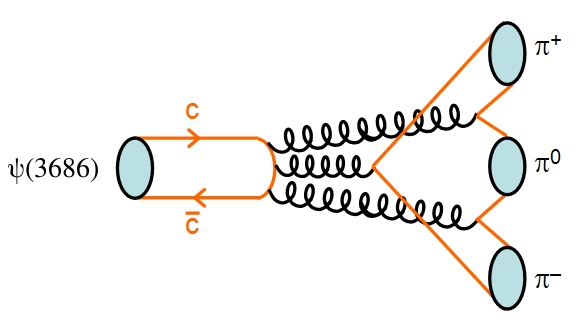
\includegraphics[scale=0.50]{figures/images/OZI_psip.png}
\caption{An example Feynman diagram for the decay of $\apsip$.}
{Without sufficient energy to produce $D$ mesons, the decays of $\apsip$ must be mediated by three hard gluons and are suppressed, as described by the OZI rule.}
\label{fig:OZI_psip}
\end{figure}

\begin{figure}[H]
\centering
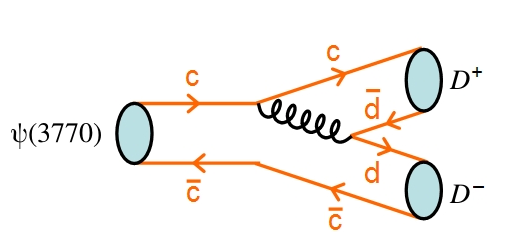
\includegraphics[scale=0.50]{figures/images/OZI_psipp.png}
\caption{An example Feynman diagram for the decay of $\psipp$.}
{With sufficient energy to produce $D$ mesons, the open-charm decays of $\psipp$ are allowed to proceed, greatly increasing the total decay width.}
\label{fig:OZI_psipp}
\end{figure}


The difference is also clearly seen in the total decay widths, where the most recent experimental averages \cite{ref:Olive:2014} are $\Gpsip = \SI{286}{\keV}$ and $\Gpsipp = \SI{27.5}{\MeV}$.
An explanation for this discrepancy was proposed independently in the 1960s by Okubo \cite{ref:Okubo:1963}, Zweig \cite{ref:Zweig:1964}, and Iizuka \cite{ref:Iizuka:1966}, and is named the OZI rule.
This states that any Feynman Diagram where the initial and final particles are separated at some point by only gluons represents a suppressed decay.
Such behavior requires that the momentum transfer from the initial particles must occur entirely through these gluons.
Because of the decreasing strength of the strong interaction with higher momentum transfer, the rate of these decays is thereby inhibited.
This is further compounded by the need for three gluons in such an interaction, as one gluon could not conserve color charge, and two could not converse $\sC$-parity.
Once above the $\DDbar$ threshold, the allowed open-charm decays dominate, and the total width is greatly increased.
This dominance points to a high branching fraction expected for decays of the type $\psipptoDD$.


\chapter{Detector and Related Systems}
\label{ch_detector}

\section{BEPCII Accelerator}

\section{BESIII Detector}

\subsection{Multi-Layer Drift Chamber}

\subsection{Time-of-Flight System}

\subsection{Electromagnetic Calorimeter}

\subsection{Muon Identifier}

\section{Triggering Systems}
\chapter{Analysis Software}
\label{ch:software}

\section{BESIII Offline Software System}

Reconstructing and processing event data gathered by the BESIII detector is done using the BESIII Offline Software System (BOSS) \cite{ref:Li:2006}.
This is an analysis software distribution written using the C++ language and running primarily on the Scientific Linux CERN operating system \cite{ref:SLC5}.
There are five main parts to BOSS: framework, simulation, reconstruction, calibration, and analysis.


\subsection{Framework}

The framework is built on the Gaudi software architecture \cite{ref:Barrand:2001}, which provides a standard interface and utilities for things such as event simulation, data processing, and physics analysis.
The software is managed using the Configuration Management Tool \cite{ref:Arnault:2000}, which provides a method for creating packages, handling package dependencies, and producing executables from source code.
There are three main filetypes for data stored by the framework: raw data ($\texttt{.raw}$), reconstructed data ($\texttt{.rec}$), and Data-Summary-Tape ($\texttt{.dst}$).
The latter two of these file types are derived from the ROOT \cite{ref:ROOT} format ($\texttt{.root}$) for easy management and usage in various analyses.


\subsection{Simulation}

There are four main parts to the simulation process: event generation, detector description, particle tracking, and detector response.
Event generation is primarily handled by the Monte Carlo (MC) generators KKMC, BesEvtGen, and Babayaga, which are described below.
To model its geometry and materials, a unique description of the detector has been created using a format based on XML.
This allows both simulation and reconstruction packages to appropriately model the behavior of events within the specific environment of BESIII.
For particle tracking, interactions with detector materials are handled by GEANT4 \cite{ref:Agostinelli:2003}.
Lastly, detector responses are modeled by the so-called `digitization code'.
This takes into account each detector component, as well as readout electronics, and realistic situations such as noise or dead channels.
There is also a simulation of the triggering system implemented.


\subsubsection{KKMC}

Originally developed for the LEP and SLC colliders, KKMC \cite{ref:Jadach:2000} is a generator used to model electroweak interactions.
Namely, the processes generated are of the form $\ee \rightarrow \ffbar + (n)\photon$, where $\fermion = \{ \mu, \tau, \qup, \qdown, \qstrange, \qcharm, \qbottom \}$, and $(n)\photon$ represents any number of additional photons.
These are modeled taking into account second-order sub-leading corrections, as well as initial-state radiation (ISR), and interference between initial- and final-state radiation (FSR).
The effects of beam energy spread, typically on the order of \SI{1}{\MeV} near the $\psipp$, can also be included.


After generation, the $\ffbar$ pair is decayed by models depending on the fermions involved.
The TAUOLA library \cite{ref:Jadach:1993} is used to decay $\tautau$ pairs, and takes into account spin-polarization effects.
The PYTHIA model \cite{ref:PYTHIA} is used to hadronize final-state $\qqbar$ continuum production using the parton shower model.
For resonances like the $\psipp$, the only action performed by KKMC is the generation of ISR.
After this, the virtual photon produced is handed off to BesEvtGen.


\subsubsection{BesEvtGen}

Originally developed for the CLEO and BaBar collaborations, EvtGen \cite{ref:Lange:2001} is another widely used generator.
It is the basis for BesEvtGen \cite{ref:Ping:2008}, which incorporates many different decay models into a single utility.
Over 30 exclusive decay models are available in BesEvtGen, as well as the capability to incorporate user-created models.


The simulation process occurs sequentially using dynamic information from decay amplitude probabilities and forward/backward spin-density matrices.
From this, final state radiation is handled by the PHOTOS model \cite{ref:Barberio:1991}.
To generate unknown decays of charmonium resonances, the LundCharm model \cite{ref:Chen:2000} is used, while other unknown hadronic decays are handled by PYTHIA.
For radiative processes, such as radiative return to $\jpsi$ or $\psip$, the VECTORISR model \cite{ref:Bonneau:1971} is used.
This occurs when one particle in the initial $\ee$ pair radiates a photon of high enough energy that only lower mass resonances can be produced from the reduced center-of-mass energy.
When the radiation is less energetic, the $\psipp$ resonance is directly produced through the combination of KKMC and BesEvtGen.


\subsubsection{Babayaga}

Production of QED processes is done using the Babayaga generator \cite{ref:Carloni:2004}.
This includes $\ee \rightarrow \{\ee, \mumu, \yy\}$.
The results are very accurate, with an estimated theoretical uncertainty of \SI{0.1}{\%}.
It also matches exact next-to-leading-order corrections from the parton shower algorithm.
The high precision is important for determination of the efficiencies and acceptances required to precisely measure the integrated luminosity.

\subsection{Reconstruction}

Reconstruction primarily involves information about specific types of particles from each of the four main detector subsystems.
These sources of information are as follows:
\begin{itemize}
    \item a charged track finding algorithm and a Kalman-filter-based track-fitter
    \item a particle identifying algorithm based on $\tdEdx$ and time-of-flight measurements
    \item a shower- and cluster-finding algorithm for EMC energy and position 
    \item a muon track finding algorithm
\end{itemize}
Further descriptions of each of these processes can be found in Sec. \ref{sec:detector_simulation}.
Additionally, algorithms for determining the corresponding beam bunch crossing, as well as for secondary vertex and track refitting, are also utilized.


\subsection{Calibration}

To maintain consistent production and analysis of datasets, a centralized source of run-dependent information is maintained by BOSS.
This includes algorithms which determine the calibration constants for each sub-detector, as well as a centralized database to store the results.
Each of the calibration outputs are stored in a ROOT file along with other details such as the beam energy, luminosity, magnetic field information, trigger conditions, and hardware/software versions.
While all of this information is stored by a central MySQL \cite{ref:MySQL} server at IHEP, other institutions in BESIII regularly synchronize with this server to create mirrored copies of these databases.



\section{Detector Simulation}
\label{sec:detector_simulation}

The following sections detail the simulation, calibration, and reconstruction processes for each detector subsystem.
Each of these relies on a geometry description created using GEANT4.


\subsection{Multi-Layer Drift Chamber}

Simulating events in the MDC accounts for axial layers, stereo layers, and endplates.
The simulation also relies on the calibration parameters to determine things such as wire efficiency and resolution as a function of drift distance for each wire, noise in each layer, and possible misalignment.


Calibration of the MDC relies on $\jpsi \rightarrow \mumu$ for both position and $\tdEdx$.
Using $\jpsi$ events allows for quickly obtaining sufficient statistics due to the very large production cross section at that peak.
The information determined includes constants such as $x-t$ relations, timing, alignment, and absolute wire efficiency.
These values are stored in the database for each run.
Special-purpose runs with the magnetic field turned off allow precise determination of wire positions.


Reconstructing MDC events starts by finding axial track segments using raw hits.
These are found by searching for matches to pre-determined patterns.
Next, these segments are fitted to circular tracks using the least-squares method.
Stereo segments are then added using an iterative helix fit.
Lastly, additional hits which were possibly missed from the initial reconstruction are added to the track using a Kalman-filter process.
This process determines the track parameters for multiple particle hypotheses.
The reconstruction is remarkably efficient, with over \SI{98}{\%} of tracks with $p_T > \SI{150}{\MeV}$ being reconstructed, even amidst high backgrounds.
From this, the charge, momentum, and trajectory can be determined for each track.


In addition to tracking, the MDC also measures the ionization energy deposited per unit length, $\tdEdx$, for each particle.
The energy deposition of each track as it passes through the chamber is compared to expectations to determine a probability for each particle hypothesis.
Corrections applied account for things such as multiple scatterings, magnetic deflection, and ionization.
This likelihood from $\tdEdx$ is combined with information from the ToF to determine the type of particle that best matches the track properties.


\subsection{Time-of-Flight System}

Simulating events in the ToF accounts for the scintillator, wrapping materials, and photomultiplier tubes (PMTs).
The process converts the energy deposited in the scintillator into photons, then propagates the shape of a photon pulse (rather than individual photons) to the PMTs in order to generate an electronic signal.
A discriminator is applied to each pulse to determine the analog-to-digital conversion (ADC) and time-to-digital conversion (TDC) outputs.
The algorithm was designed and tested with dedicated test beam data, however, each new data set requires updated tuning.
A full simulation tracing each optical photon is also available for detailed study of the timing measurements.


Calibration of the ToF also uses $\jpsi$ decays to dileptons for both timing and energy measurements.
The information determined includes effective velocity, attenuation length, and muon energy loss.
The status and performance of the ToF are regularly monitored by a laser-fiberoptics pulsing system.


Reconstructing ToF events starts by using tracks with trajectories extrapolated from the MDC.
Each track is matched with a particular ToF module; either the two layers of the barrel, or the single-layer endcap.
The travel time for each hypothesis is then calculated using weighted-average times from PMTs at both ends of the scintillator.
Corrections are also applied to account for aspects like the effective light velocity in the scintillator and the light attenuation length.
Measurements of deposited energy are obtained for both charged and neutral particles, and are added to the EMC to improve the shower energy resolution.


\subsection{Electromagnetic Calorimeter}

Simulating events in the EMC accounts for the crystals, casing, silicon photodiodes, preamplifier boxes, cables, and the support system.
For each of the crystals and photodiodes, hit information is recorded, and the deposited energy is summed.
From this, photon statistics are computed, and the resulting photodiode response is converted into electronic signals.
To obtain the waveform in the time domain, an inverse Laplace transform is applied.
Then, a sampling and peak searching process is simulated to yield energy and time information.
For each bin, Gaussian-type electronic noise is added, and the background is produced by summing over the waveforms.


Calibration of the EMC uses Bhabha electrons with $E > \SI{1.55}{\GeV}$ for the high energy response, and $\piO \rightarrow \yy$ decays for the low energy response.
The responses for individual crystals must be analyzed separately, due to their potential intrinsic variations.
As a result, they are monitored frequently by a LED light pulser, and periodically recalibrated.
Corrections due to temperature variations are also applied.


Reconstructing EMC events starts by converting the ADC value of each crystal into energy based on the calibration constants.
After this, clusters in both the barrel and endcaps are formed by analyzing local maximum energy deposits, called seeds.
A clustering algorithm then aggregates hits around these seeds and sums the values for a particular shower.
The position of each shower is then calculated using the energy-weighted first moment.
If multiple seeds are found in one cluster, a splitting algorithm is invoked to split the cluster into multiple showers.
Additionally, matching energy deposits from the ToF are also added back into the total shower energy.
This improves the energy resolution, particularly for low energy photons.


\subsection{Muon Identifier}

Simulating events in the MUC accounts for forming each RPC, creating sets of strips to form each read-out plane, combining each of these with aluminum boxes to form a muon counter module, and interleaving the modules between layers of iron plates.
The digitization from the read-out planes is selected to fire based on the distance to each track.
Noise is simulated using Poisson distributions initially determined from measurements made during the construction of the chamber, and updated during actual data taking.


Calibration of the MUC analyzes RPC detection efficiencies as function of area.
The cluster sizes and noise levels are also studied.


Reconstructing MUC events starts by searching for collected hits in each of the barrel and endcap orientations.
The two collections are then matched with reconstructed tracks from the MDC.
Since low momentum muons may cause only a few layers to fire, a subsequent search is performed over unused hits based on the extrapolated trajectories of MDC tracks.
The reconstruction process primarily analyzes the depth of the track in the MUC, the maximum number of hits in the layers fired by a track, and the matching between a MDC track with the MUC stand-alone track.
These parameters, along with the track momentum and MDC exit angle, are input into an Artificial Neural Network in order to distinguish between hadron and muon tracks.
The identification process is quite effective, generally removing \SI{\sim96}{\%} of pions and retaining \SI{\sim90}{\%} of muons.



\section{$D$-Tagging}
\label{sec:d_tagging}

From the decay of the $\psipp$, the most commonly produced particles are $\DO\aDO$ or $\Dp\Dm$ pairs.
Since the $\DDbar$ pairs are produced in two-body decays, the energy of each $\D$ is half of the center-of-mass energy (in the center-of-mass reference frame).
Each of these $\D$ mesons then quickly decays to certain sets of particles.
Reconstructing one of these decays requires assembling the right combination of such particles under the constraint of 4-momentum conservation.


This reconstruction technique is known as `$\D$-Tagging', and was pioneered by the MARK-III collaboration \cite{ref:Baltrusaitis:1986,ref:Adler:1988}.
For our analysis, the particles analyzed in the detector include $\pipm, \Kpm, \piO,$ and $\Ks$, and the decay modes used are shown in \Cref{tab:dtag_modes}.
There are three $\DO$ modes and six $\Dp$ modes, where charge conjugation (converting all particles to their anti-particles) is implied throughout the analysis.
The modes used are chosen for their overall efficiency of reconstruction in the detector; they generally have higher branching fractions and manageable multiplicity (the number of tracks in the final state).
For the neutral modes, this procedure also includes the doubly-Cabbibo suppressed decays (DCSD), such as $\DO \rightarrow \Kp \; \pim$, which have small and well-measured branching fractions.

\begin{table}[h]
\centering
\begin{tabular}{l|l l}
\hline
(0) $\DOmodeA$ & (200) $\DpmodeA$ & (203) $\DpmodeD$ \\
(1) $\DOmodeB$ & (201) $\DpmodeB$ & (204) $\DpmodeE$ \\
(3) $\DOmodeC$ & (202) $\DpmodeC$ & (205) $\DpmodeF$ \\
\hline
\end{tabular}
\caption{The reconstructed $\Dtag$ modes used in this analysis.}
{The numerical values are shorthand codes used by the reconstruction software.}
\label{tab:dtag_modes}
\end{table}

This process occurs for each event and searches over each decay mode for each charm state ($\Dp$ and $\Dm$).
The combinations chosen for reconstruction are those with the smallest energy difference from the expected value.
More than one $\D$ combination can be extracted from a given event, as long as it satisfies all other requirements (see \Cref{ssec:selection_cuts}).
While this may sound like it overestimates the number of actual $\D$ particles found, the process is also used to calculate reconstruction efficiency, thereby eliminating any bias.


\subsection{Selection Cuts}
\label{ssec:selection_cuts}

Before being considered as potential reconstruction candidates, each track in the detector must also pass other cuts specific to its identified particle type.
The following describes the criteria required for the particles in the decay modes we are using.


\subsubsection{$\pipm / \Kpm$ Selection}
\label{sssec:kpi_selection}

Each of the reconstructed charged tracks must pass vertex cuts in both the transverse ($x-y$) and beam ($z$) directions relative to the interaction point.
This requires that tracks originate sufficiently close to the interaction point to ensure they are not other backgrounds, such as cosmic rays, or daughters of tracks which have decayed in flight.
There is also a cut on the polar angle measured within the MDC ($\theta$) to ensure the track can reliably be reconstructed.
Lastly, from the particle identification process, the probability of being a pion (kaon) must be greater than that for being a kaon (pion).
The specific cuts for each of these requirements can be found in \Cref{tab:kpi_cuts}.

\begin{table}[h]
\centering
\begin{tabular}{c| r@{$\; < \;$}l }
\hline
Vertex ($xy$)    & $V_{xy}$ & \pp \SI{1}{\cm} \\
Vertex ($z$)     & $|Vz|$   & \SI{10}{\cm} \\
MDC Angle        & $|\cos\theta|$ & 0.93 \\
Pion Probability & \multicolumn{2}{c}{ $\pp P(\pi) > 0, \quad P(\pi) > P(K)$ } \\
Kaon Probability & \multicolumn{2}{c}{ $P(K)   > 0, \quad P(K) > P(\pi)$ } \\
\hline
\end{tabular}
\caption{The required cuts to identify charged tracks as $\pipm$ or $\Kpm$.}
\label{tab:kpi_cuts}
\end{table}


\subsubsection{$\photon$ Selection}
\label{sssec:photon_selection}

To distinguish photon energy from noise, each shower in the EMC is required to have a certain amount of deposited energy.
These cuts are different for the barrel ($|\cos\theta| < 0.80$) and endcap ($0.84 < |\cos\theta| < 0.92$) regions.
Each photon must also pass a timing cut to ensure they are consistent with actual physics events, and not originating at other times.
The values for each of these requirements can be found in \Cref{tab:photon_cuts}.

\begin{table}[h]
\centering
\begin{tabular}{c|c r}
\hline
Minimum Energy (Barrel) & $E_{\text{EMC}} > \SI{25}{\MeV}$ & $(|\cos\theta| < 0.80)$ \\
Minimum Energy (Endcap) & $E_{\text{EMC}} > \SI{50}{\MeV}$ & $(0.84 < |\cos\theta| < 0.92)$ \\
TDC Timing & $ (0 \leq t \leq 14) \times \SI{50}{\ns} $ \\ 
\hline
\end{tabular}
\caption{The required cuts to identify neutral showers as a $\photon$.}
\label{tab:photon_cuts}
\end{table}


\subsubsection{$\piO$ Selection}
\label{sssec:pi0_selection}

Reconstructing $\piO$ mesons involves finding $\yy$ pairs, as this the most dominant decay (\SI{\sim99}{\%}).
Each of the $\photon$ showers must pass the cuts described above. 
Additionally, at least one photon in the pair must be found in the barrel region.
Each of the two photons are then kinematically fitted to compare with the invariant mass of the $\piO$, and must also pass a proper fit cut.
The resulting momentum from this fit is used for reconstructing $\Dtag$ candidates.
The values used for each of these requirements are shown in \Cref{tab:pi0_cuts}.

\begin{table}[h]
\centering
\begin{tabular}{c|c}
\hline
Nominal Mass & $\SI{115}{\MeV} < m_{\piO} < \SI{150}{\MeV}$ \\
Fit Quality  & $\chi^2 < 200$, Converged \\
\hline
\end{tabular}
\caption{The required cuts to reconstruct $\yy$ pairs as a $\piO$.}
\label{tab:pi0_cuts}
\end{table}


\subsubsection{$\Ks$ Selection}
\label{sssec:ks_selection}

Reconstructing $\Ks$ mesons involves finding $\pip\pim$ pairs, as this is its most common decay (\SI{\sim70}{\%}).
While $\piO\piO$ pairs are also a substantial decay mode (\SI{\sim30}{\%}), these are not considered due to the difficulty of correctly reconstructing the $4\photon$ final state.
To account for the $\Ks$ decaying in flight, each of the charged pions considered are not subjected to the vertex or probability cuts in \Cref{tab:kpi_cuts}.
Instead, the two found pions are kinematically constrained to a common vertex.
The results must pass a nominal mass cut (\SI{\sim3}{\sigma}) and a proper fit cut to be deemed a $\Ks$.
From this, the resulting momentum from the vertex fit is used for reconstructing $\Dtag$ candidates.
The values used for each of these requirements are shown in \Cref{tab:ks_cuts}.

\begin{table}[h]
\centering
\begin{tabular}{c|c}
\hline
Nominal Mass & $\SI{487}{\MeV} < m_{\Ks} < \SI{511}{\MeV}$ \\
Fit Quality  & $\chi^2 < 100$, Converged \\
\hline
\end{tabular}
\caption{The required cuts to reconstruct $\pip\pim$ pairs as a $\Ks$.}
\label{tab:ks_cuts}
\end{table}

\subsubsection{Cosmic Ray and Lepton Veto}
\label{sssec:cosmic_and_lepton}

When reconstructing the mode $\DOmodeA$, an additional veto is used.
Since this mode has only two charged tracks, it is common to misidentify particles which come from cosmic ray and backgrounds like $\ee \rightarrow \{\gamma\ee, \; \gamma\mumu\}$.
To prevent this, cuts on the timing difference between the tracks, as well as on the particle identification variables, are imposed.
The values used for these requirements are shown in \Cref{tab:veto_cuts}.

\begin{table}[h]
\centering
\begin{tabular}{c|c}
\hline
Timing (TDC) & $|t_1 - t_2| < 5 \times \SI{50}{\ns}$ \\
Particle Identification & $(\chi_{\lel}^2 + \chi_{\alel}^2) - (\chi_{\Km}^2 + \chi_{\pip}^2) > 10$ \\
\hline
\end{tabular}
\caption{Cuts to suppress cosmic ray and lepton backgrounds in $\DOmodeA$.}
\label{tab:veto_cuts}
\end{table}


\subsection{Reconstruction}
\label{ssec:dtag_reconstruction}

After all of the constituent particles are identified, reconstructed $\D$ candidates are characterized by two main kinematic quantities:
\beq
\DeltaE = |\Ebeam - \Etag|, \qquad \qquad \mbc = \sqrt{\Ebeam^2 - |\ptag|^2}.
\eeq
These are the energy difference ($\DeltaE$) and the beam-constrained mass ($\mbc$), and effectively represent the energy and momentum of the $\Dtag$, respectively.
As the candidate with the smallest $\DeltaE$ for each decay mode in each event is selected, the values will peak near \SI{0}{\MeV}.
Distributions of $\mbc$ peak near the respective $D$ masses, $m_{\DO} = \SI{1.865}{\GeV}$ or $m_{\Dp} = \SI{1.870}{\GeV}$.
While invariant mass ($\minv = \sqrt{\Etag^2 - |\ptag|^2}$) is an alternative selection variable, $\mbc$ is preferred because the beam energy is more precisely known than the 4-momenta of the individual particles comprising the $D$ candidate.


%
%% Analysis Chapters
%\include{chapters/data_set}
%\include{chapters/event_selection}
%\include{chapters/analysis}

% Conclusion
\chapter{Conclusion}
\label{ch_conclusion}

This is where the Conclusions go!

% Bibliography
\bibliography{references}

% Appendices
\appendix
\chapter{Glossary and Acronyms}
\label{app_glossary}

Care has been taken in this thesis to minimize the use of jargon and
acronyms, but this cannot always be achieved.  This appendix defines
jargon terms in a glossary, and contains a table of acronyms and their
meaning.

% Glossary {{{
\section{Glossary}
\label{sec_glossary}

\begin{itemize}

\item \textbf{Cosmic-Ray Muon} (\textbf{CR $\mu$}) -- A muon coming from
the abundant energetic particles originating outside of the Earth's
atmosphere.

\end{itemize}


% Acronyms {{{
\section{Acronyms}
\label{sec_acronym}

% Table formatting

% Heading for the first page
\begin{longtable}{p{0.25\textwidth} p{0.75\textwidth}}
\caption{Acronyms} \label{tab:acronyms} \\

\toprule
Acronym & Meaning \\
\midrule
\endfirsthead

% Heading for all subsequent pages
\multicolumn{2}{l}{\textit{\tablename\ \thetable{} -- Continued from previous page}} \\
\toprule
Acronym & Meaning \\
\midrule
\endhead

% Footer for each page that wraps over to the next
\multicolumn{2}{r}{\textit{Continued on next page}} \\
\bottomrule
\endfoot

% Footer for the end of the table
\bottomrule
\endlastfoot

% End table formatting

CR$\mu$ & Cosmic-Ray Muon \\

\end{longtable}


\end{document}
